%File: formatting-instruction.tex
\documentclass[letterpaper]{article}
\usepackage{aaai}
\usepackage{times}
\usepackage{helvet}
\usepackage{courier}
\usepackage{amsmath}
\usepackage{amsfonts}
\usepackage{graphicx}
\usepackage{hyperref}
\usepackage{xcolor}

\frenchspacing
\setlength{\pdfpagewidth}{8.5in}
\setlength{\pdfpageheight}{11in}
\pdfinfo{
/Title (Collaboration and Competition Project Report)
/Author (Piero Macaluso)}
\setcounter{secnumdepth}{0}  
 \begin{document}
% The file aaai.sty is the style file for AAAI Press 
% proceedings, working notes, and technical reports.
%
\title{Collaboration and Competition Project Report}
\author{Piero Macaluso}
\maketitle

\section{Introduction}

The purpose of this document is to briefly present the work done in this project, along with the algorithm used and implemented, but also with a showcase of the results obtained.

This document can be divided into 4 parts:

\begin{itemize}
\item \textbf{Introduction}: the current section;
\item \textbf{Learning Algorithm}: an overview of the approaches and methods used to solve the problem;
\item \textbf{Results}: a presentation of the results reached with plots and GIFs of the best episodes;
\item \textbf{Future Work}: some ideas on how to improve the actual algorithm.
\end{itemize}

\section{Learning Algorithms}

The \textit{Tennis} environment consists of 2 agents in competition that interacts simultaneously with the environment.

The chosen algorithm was the Multi Agent Deep Deterministic Policy Gradient (MADDPG) one \cite{lowe2017multi}. MADDPG is general-purpose multi-agent learning algorithm that leads to learned
policies that only exploit local information at execution time (i.e. their observations). In addition, it does not assume a specific communication method between agents, and is applicable to cooperative, competitive and mixed interactions.

As presented in Figure \ref{fig:maddpg}, the authors of \cite{lowe2017multi} proposed an extension of actor-critic policy gradient methods where the critic is augmented with extra information about the policies of other agents, while the actor only has access
to local information. After the completion of the training process, the algorithm only uses local actors at execution phase: this fact makes this technique equally applicable in cooperative and competitive settings.

In the context explained, the policies of other agents are needed to apply an update in Eq. \ref{eq:maddpgloss}. Knowing the observations
and policies of other agents is not a particularly restrictive assumption. Our goal is to train agents to exhibit complex communicative behaviour in simulation, therefore this information is often available to all
agents.

\begin{equation}\label{eq:maddpgloss}
	\begin{gathered}
		\mathcal{L}(\theta_i) = \mathbb{E}_{x,a,r,x'}[(Q_i^{\mu}(x,a_1, \dots,a_N)-y)^2] \\
		y_t = r_i + Q_i^{\mu'}(x',a'_1, \dots,a'_N)|_{a'_j=\mu'_j(o_j)}
	\end{gathered}
\end{equation}

It is clear from Equation \ref{eq:maddpgloss} that the loss is calculated starting from experiences sampled from a \textit{replay buffer} that gathers all the past experiences of all agents. Therefore, $Q_i^\pi(x,a_1, \dots,a_N)$ is a centralized action-value function that takes as input the actions of all agents in addition to some state information x, and outputs the Q-value for agent $i$.

\begin{figure}[h!]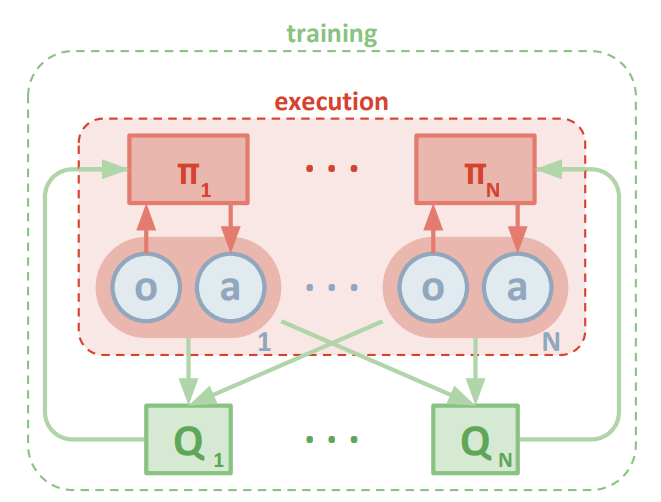
\includegraphics[width=\linewidth]{img/maddpg.png}
\caption{Overview of the multi-agent decentralized actor, centralized critic approach presented in \cite{lowe2017multi} \label{fig:maddpg}}
\end{figure}   

\subsection{Hyper-parameters}

The environment state and action space is very simple and it does not require convolutional neural networks. For this reason, both the actor and the critic were implemented with 2 fully connected layer with 128 neurons as hidden size. Both networks exploits \textit{Leaky Rectified Linear Unit} (LeakyReLU) as non-linearity for each layer. The policy uses Tanh as non-linearity for the last layer, while the critic does not use non-linearity for the last layer.

There is a difference between the critic used in the DDPG framework and the ones we used in this context. This time, we put as input the concatenation of states and actions of all agents.
The hyper-parameters used are presented in Table \ref{table:hp}.

Taking into account the work done in the previous project, we added to the algorithm \textit{gradient clipping} for the critic, \textit{weight initialization} for both networks and avoided the usage of \textit{batch normalization}.
For what concerns the noise, we decided to implement a degradation of the $\sigma$ parameter until a minimum of $0.01$ with a noise decay equal to $0.9995$.

\begin{table}[]
\begin{tabular}{rl}
\textbf{Hyper-parameters}    & \textbf{Value}        \\
Memory Buffer Size          & $10^6$ \\
Batch Size                  & $256$                    \\
Gamma                       & $0.99$                  \\
Tau                         & $10^{-3}$                 \\
Learning Rate               & $1\times 10^{-3}$                  \\
Learning Frequency          & $2$ (as \#agent) updates per steps       \\
Target Update Frequency        & every $2$ (as \#agent) learning steps           \\

Ornstein-Uhnlebeck Noise &  $\theta=0.15$, $\sigma=0.20$ decaying
\end{tabular}
\caption{Hyper-parameters used in the training process}
\label{table:hp}
\end{table}

\section{Results}

The number of episodes to play was fixed at $2000$ and the agent took just $1826$ episodes to reach an average score on the last 100 episodes using the maximum reward over the 2 agents greater than $0.5$. The highest average score on the last 100 episodes was equal to $1.36$ reached at episode $2000$.

To find the best solution, a test phase of 10 episodes was implemented and started every 50 training episodes to evaluate the results without taking into account exploration noise. As shown in Figure \ref{fig:plot}, the best test result was found at episode $2000$ \footnote{GIF reporting a handful of seconds of the testing phase \href{https://raw.githubusercontent.com/pieromacaluso/collaboration-n-competition/14820105ae05007df12a2a844f34532779916151/stuff/solved_gif.gif}{\textcolor{blue}{here}.}} with an average of $2.29$ over 10 episodes.

\begin{figure}[h!]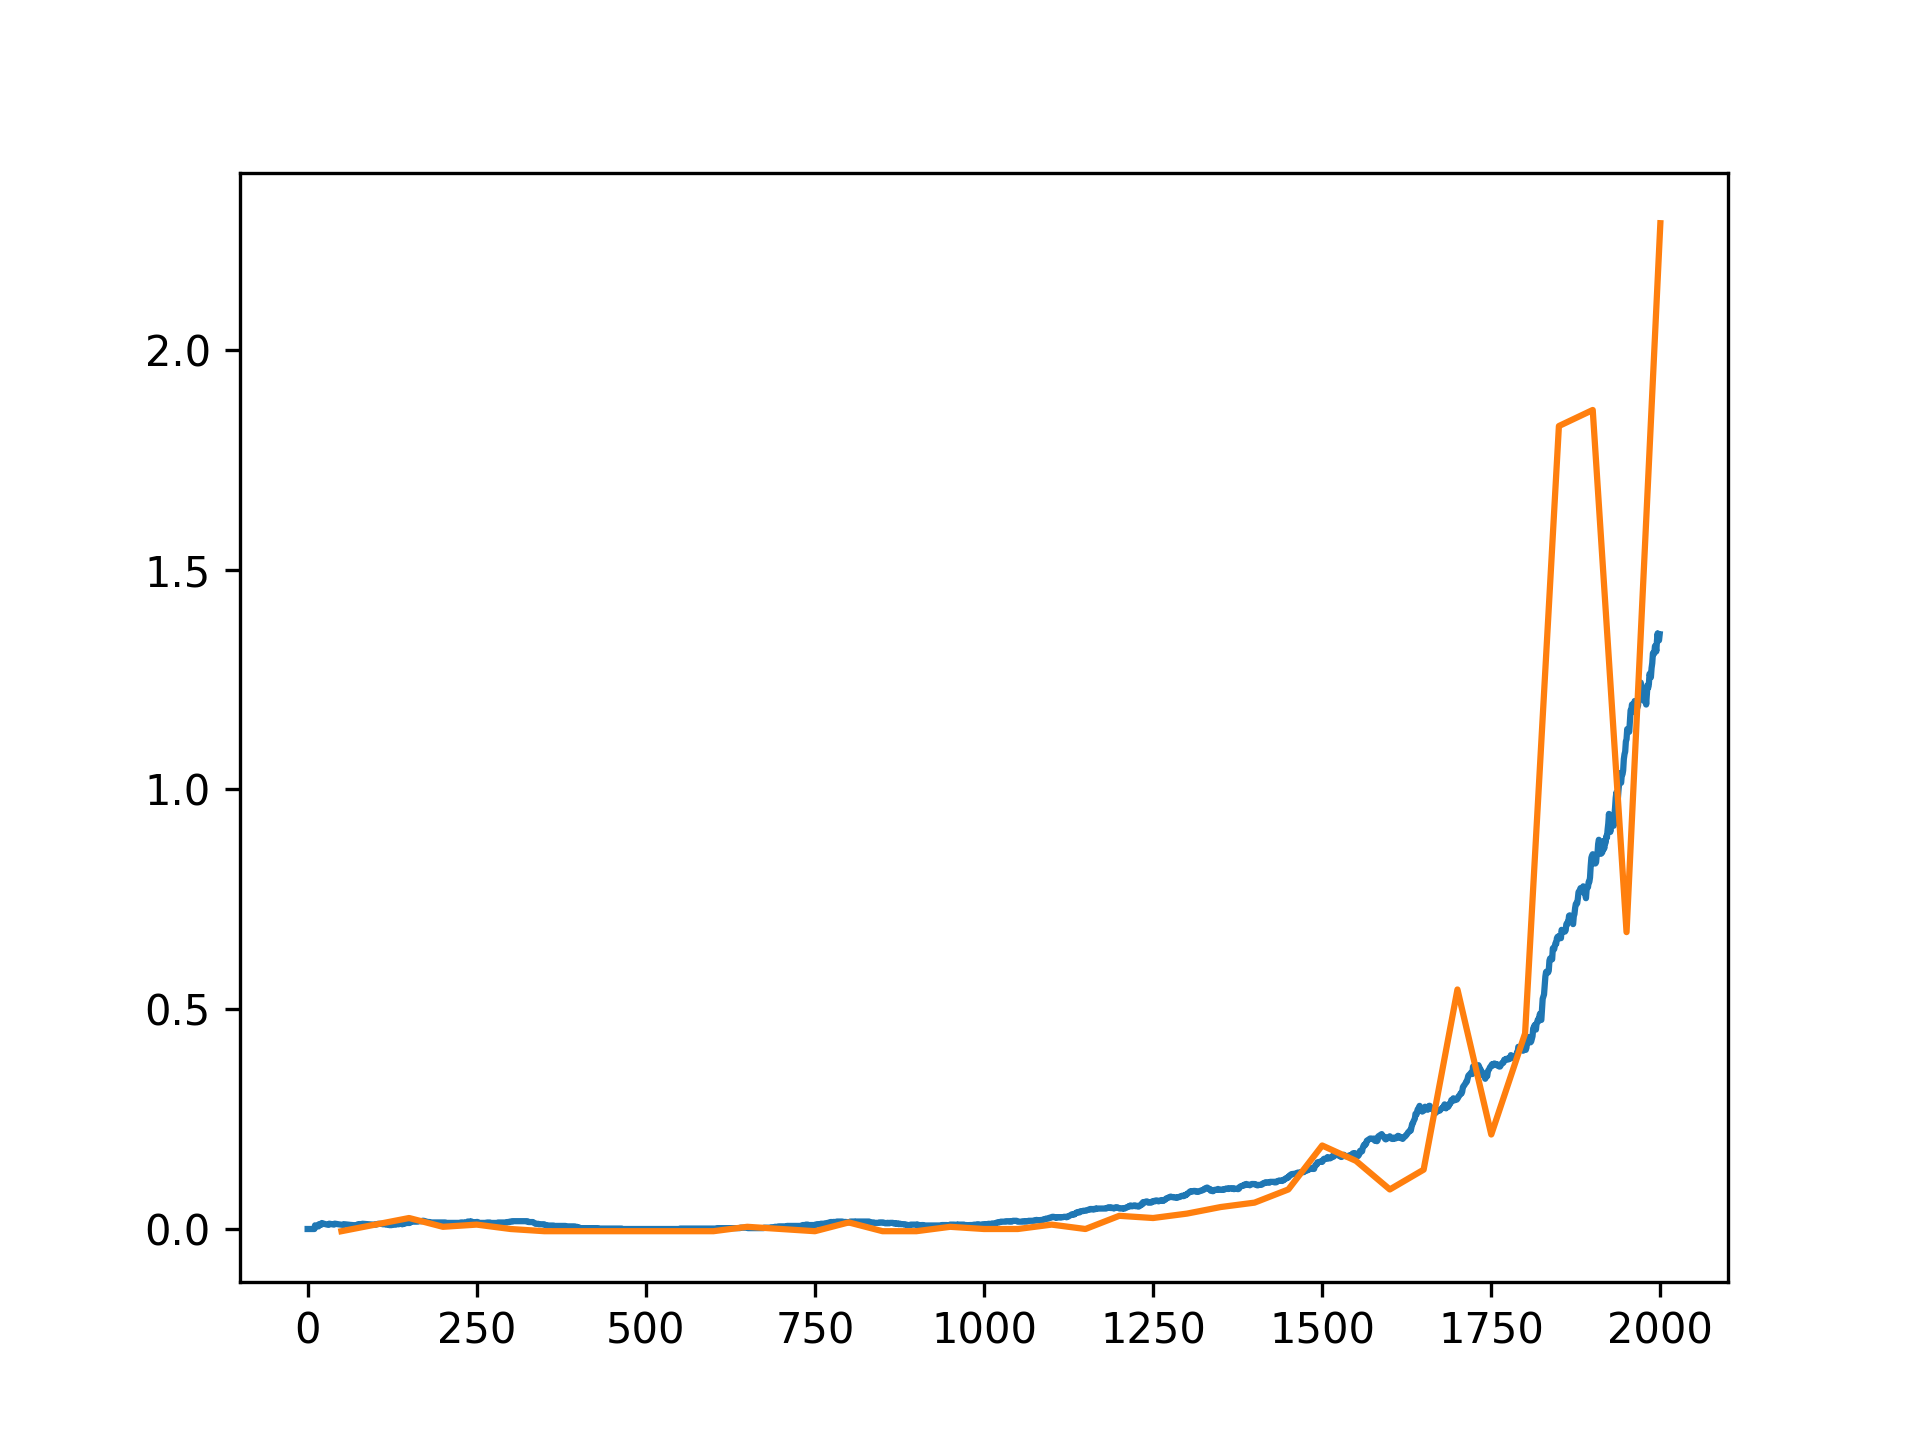
\includegraphics[width=\linewidth]{img/avg.png}
\caption{Training (blue) and Test (orange) Scores History\label{fig:plot}}
\end{figure}   

\begin{figure}[]
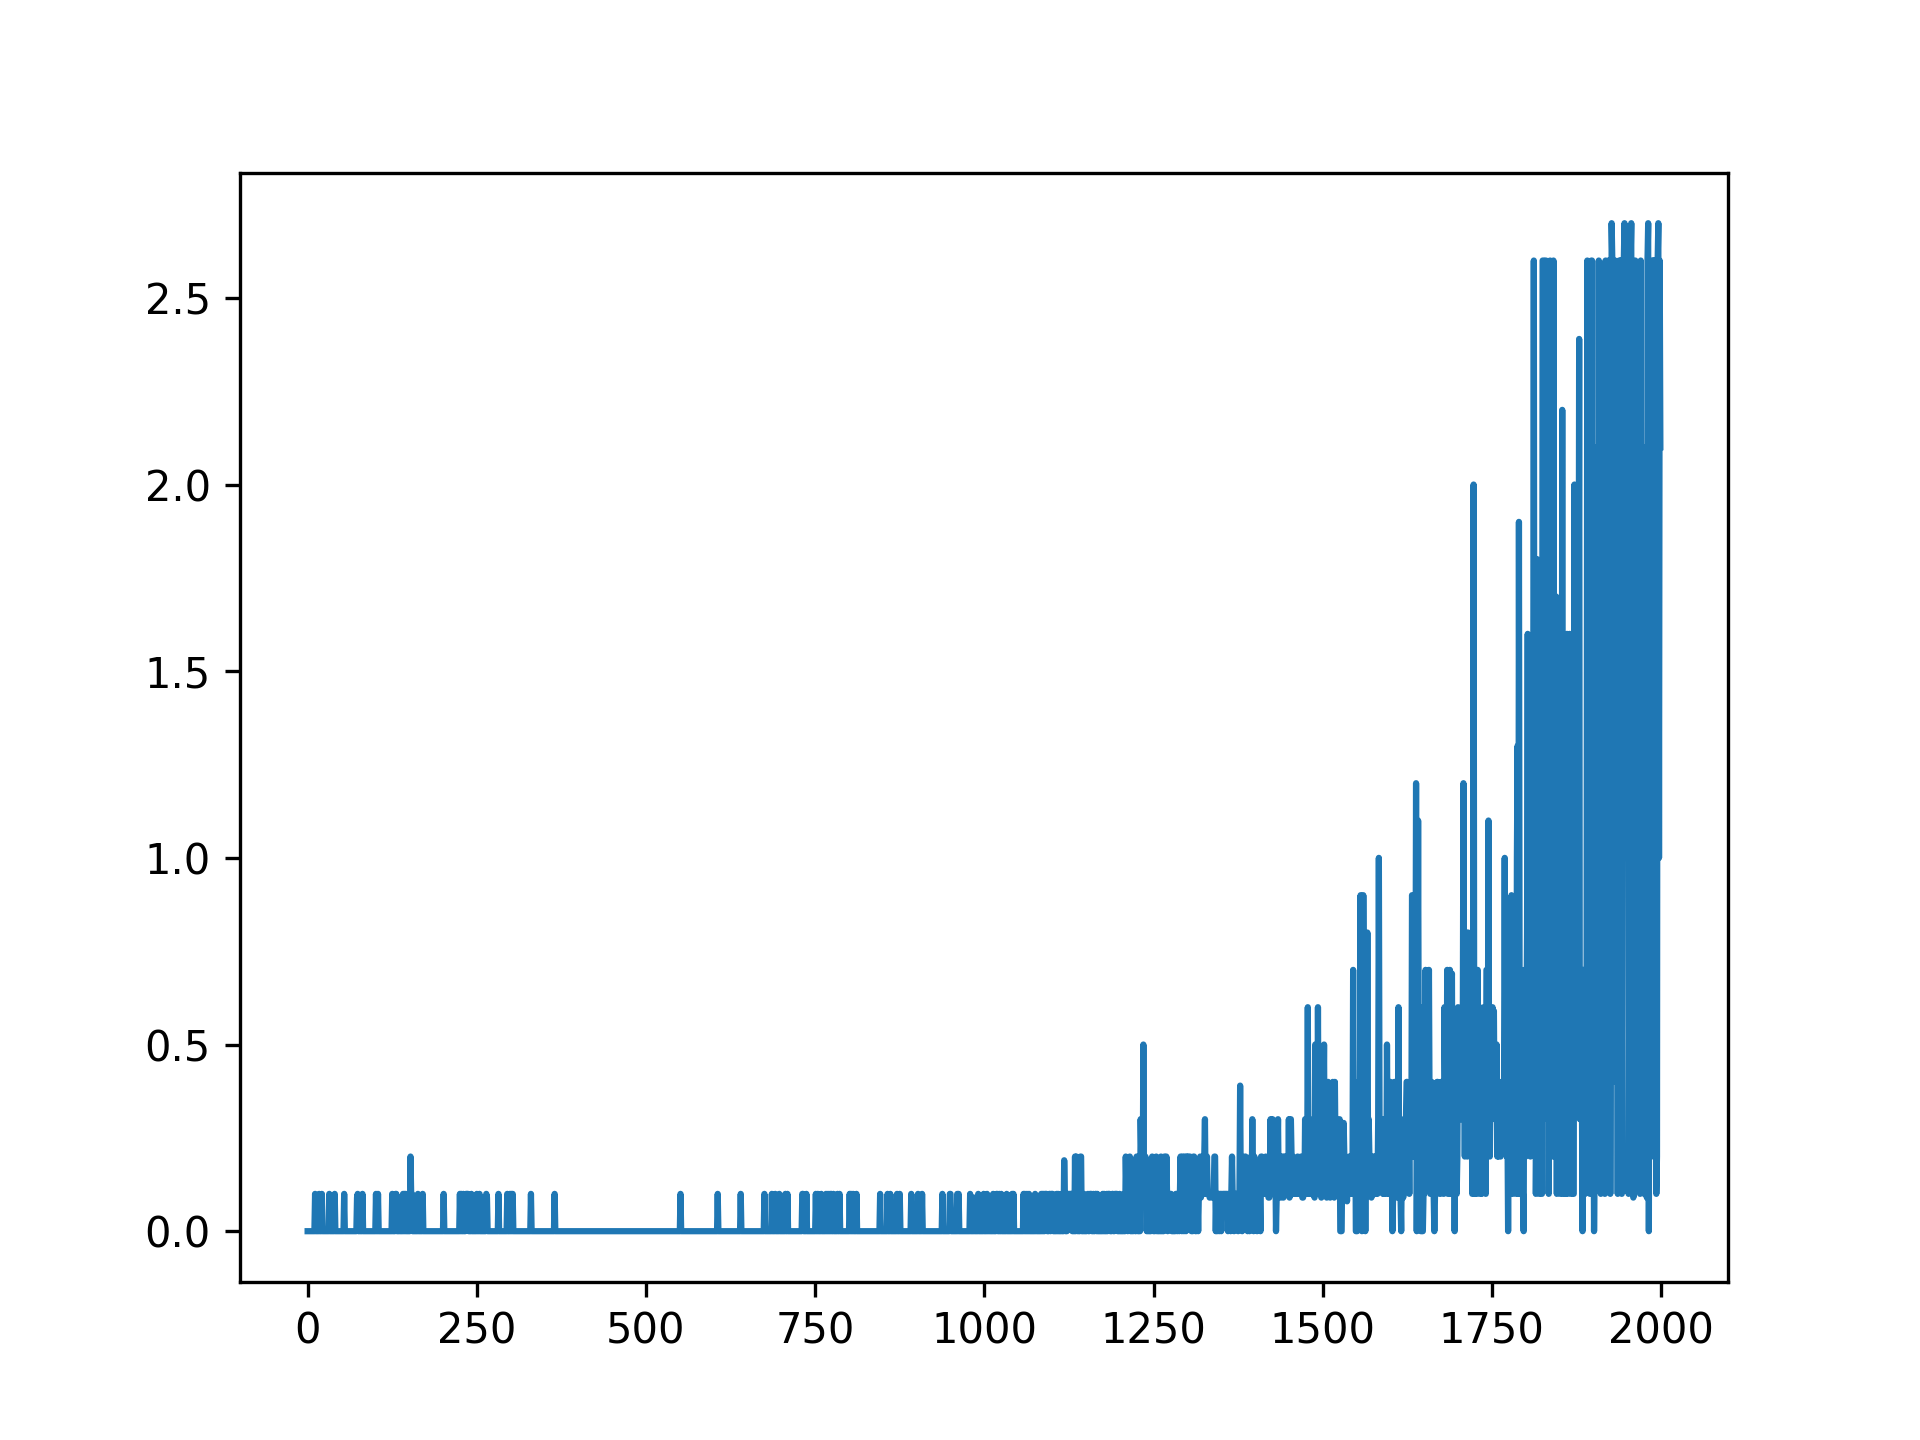
\includegraphics[width=\linewidth]{img/scores.png}
\caption{Training Scores of all 20 agents\label{fig:plot2}}
\end{figure}   

\section{Future Work}

The results obtained were very encouraging and positive, the agents managed to improve their behaviour with stability. Possible improvements ranges from the usage of Noisy Layers instead of Action Noise \cite{fortunato2017noisy} to  training agents with an ensemble of policies \cite{lowe2017multi}.


\bibliographystyle{aaai}
\bibliography{bibliography}
\end{document}